%%
%% IJHCS Paper Draft
%% Active Questioning Strategies for Household Rearrangement
%%
\documentclass[a4paper,fleqn]{cas-sc}

\usepackage[authoryear,longnamesfirst]{natbib}
\usepackage{amsmath,amssymb}
\usepackage{booktabs}
\usepackage{multirow}
\usepackage{graphicx}
\usepackage{xcolor}
\usepackage{enumitem}

% Placeholder command for sections not yet written
\newcommand{\TODO}[1]{\textcolor{red}{\textbf{[TODO: #1]}}}

\begin{document}
\let\WriteBookmarks\relax
\def\floatpagepagefraction{1}
\def\textpagefraction{.001}

\shorttitle{Active Questioning Strategies for Household Rearrangement}

\shortauthors{Anonymous et al.}

\title[mode=title]{How Should a Robot Ask? Comparing Active Questioning Strategies for Learning User Preferences in Household Rearrangement}

% Authors placeholder
\author[1]{Anonymous Author One}
\cormark[1]
\ead{anonymous@university.edu}
\affiliation[1]{organization={Anonymous University},
            city={City},
            country={Country}}

\cortext[1]{Corresponding author}

% ============================================================
% ABSTRACT
% ============================================================
\begin{abstract}
Household tidying is a deeply personal activity shaped by individual habits, mental categories, and tacit organizing principles that users rarely articulate unprompted. When an intelligent agent assists with rearrangement, the central challenge is not \emph{what} to learn but \emph{how to ask}---whether to query individual object placements, elicit category-level rules, or confirm patterns inferred from prior evidence. We identify three complementary questioning patterns operating at different granularities---\textbf{Action-Oriented} (AO), \textbf{Preference Eliciting} (PE), and \textbf{Preference Induction} (PI)---and compose them into four dialogue policy modes that differ in \emph{when} and \emph{how} patterns are deployed. We implement these within an LLM-based conversational agent and evaluate them through a large-scale simulation across 102 household episodes with question budgets from 1 to 10. Our primary finding is that \emph{how} an agent asks matters as much as \emph{how many} questions it asks: the User-Preference-First policy (PE then AO) achieves 69.8\% unseen-object accuracy at budget 5---11.1 percentage points above Direct Querying (AO only)---because category-level rules transfer directly to novel objects. Notably, a bottom-up do-and-induce policy (AO then PI) fails to outperform direct querying, revealing that the value of preference rules depends critically on how they are acquired: top-down elicitation is far more efficient than bottom-up induction. Cross-model validation with GPT-5 preserves the policy ranking while amplifying the preference-first advantage to +15pp. Study~2, a controlled user study, is designed to examine how questioning strategies affect perceived control, cognitive load, and satisfaction, with organizing expertise as a moderating variable.
\end{abstract}

\begin{highlights}
\item Four dialogue policy modes compose three questioning patterns with distinct accuracy profiles
\item Preference-first policy achieves +11pp unseen accuracy over direct querying across 102 episodes
\item Bottom-up rule induction fails to outperform direct querying, revealing elicitation efficiency matters
\end{highlights}

\begin{keywords}
active questioning \sep preference learning \sep household rearrangement \sep conversational agent \sep large language models \sep user study
\end{keywords}

\maketitle

% ============================================================
% 1. INTRODUCTION
% ============================================================
\section{Introduction}\label{sec:intro}

Organizing a home is a skill shaped by personal habit. Two people sharing the same kitchen may sort identical objects along entirely different principles---one by function (``cooking tools near the stove''), another by frequency of use (``daily items at eye level''), a third by aesthetics (``everything visible must match in colour''). These principles are rarely written down or easily verbalized; they emerge from years of practice and tend to feel obvious to the person who holds them. Yet for an intelligent agent tasked with assisting in household rearrangement, the task is precisely to surface these tacit preferences---quickly, unobtrusively, and correctly---before placing objects on the user's behalf.

The central interaction design challenge is not whether to ask, but \emph{how}. An agent operating under a limited question budget must choose between asking about specific objects (``Where should the wireless speaker go?''), eliciting category-level rules (``How do you usually organize electronic accessories?''), or confirming patterns it has inferred from earlier answers (``I've noticed you place books on the display shelf---is that a general rule?''). These choices are not merely technical: they reflect assumptions about how users represent their own preferences, what abstraction levels they can comfortably reason about, and how much control they expect to retain over the organizing decisions.

Prior work on conversational agents has shown that the form of a question---not just its content---significantly shapes the quality of the answer it elicits and the user's experience of the interaction \citep{jin2024way}. In task-oriented dialogue, the tension between task efficiency and relational quality mirrors the tension between information-dense category questions and simpler object-level queries \citep{haugeland2022understanding}. Yet despite this established sensitivity to dialogue strategy, the question of how intelligent agents should ask for \emph{personal preferences}---especially at different granularities---has not been systematically studied.

This paper addresses that gap by investigating three active questioning strategies---\emph{Action-Oriented} (AO), \emph{Preference Eliciting} (PE), and \emph{Preference Induction} (PI)---that differ in the cognitive demands they place on users and the type of preference knowledge they target. We pursue four research questions:

\begin{enumerate}[label=\textbf{RQ\arabic*:},leftmargin=*]
    \item How does dialogue policy---the composition and sequencing of questioning patterns---affect generalization to unseen objects across different question budgets?
    \item Does top-down preference elicitation (PE) provide measurable generalization benefits over bottom-up preference induction (PI) from the same questioning budget?
    \item How do the policies differ in their effects on perceived control, cognitive load, satisfaction, and trust in the agent?
    \item Do individual characteristics---specifically, users' prior organizing expertise---moderate the relative effectiveness of different policies?
\end{enumerate}

To address RQ1 and RQ2 at scale, we conduct a large simulated evaluation (Study~1) using LLM-grounded oracles across 102 annotated household episodes at budgets 1--10. To address RQ3 and RQ4, we conduct a controlled user study (Study~2) with real participants. The convergence and divergence between simulation and user study results reveals which aspects of preference communication can be approximated computationally and which require human participants.

Our contributions are:

\begin{itemize}[leftmargin=*]
    \item A \textbf{taxonomy of three questioning patterns and four dialogue policies} for preference learning in household rearrangement, formalized along the dimensions of target granularity, cognitive demand, generalization scope, and pattern composition.
    \item An \textbf{LLM-based agent implementation} with pattern-specific proposers, a structured preference state, and a policy controller that composes patterns according to each policy mode's strategy, enabling rigorous per-policy evaluation.
    \item \textbf{Simulation findings} across 102 episodes demonstrating that preference-first questioning (UPF) achieves +11pp unseen accuracy over direct querying, while bottom-up induction (PAR) fails to outperform it---revealing that the \emph{acquisition method}, not just the presence of rules, determines generalization benefit. Cross-model validation with GPT-5 preserves the policy ranking.
    \item A \textbf{controlled user study} designed to characterize the accuracy--agency trade-off across policies and test whether organizing expertise moderates their relative effectiveness, with implications for adaptive policy selection.
\end{itemize}


% ============================================================
% 2. RELATED WORK
% ============================================================
\section{Related Work}\label{sec:related}

\subsection{Dialogue Strategy in Human-Agent Interaction}

How an agent structures its questions has well-documented consequences for user behavior and experience. \citet{haugeland2022understanding} compared topic-led and task-led conversation strategies in service chatbots (n=35), finding that topic-led approaches enhance perceived anthropomorphism and hedonic quality while task-led designs improve pragmatic outcomes---a tension that maps directly onto our comparison of category-level (PE) and object-level (AO) questioning. \citet{jin2024way} showed that conversation-based questioning outperforms form-based questioning for eliciting detailed user responses, with credibility as a significant mediator; their 2$\times$3 design underscores that the \emph{form} of the question---not just its content---shapes what users reveal.

These findings motivate our core research design: rather than comparing fixed-content questions, we compare qualitatively different questioning strategies---strategies that differ in what cognitive operations they demand of users. The existing literature demonstrates that such differences matter; it does not yet tell us which strategy granularity best serves the specific challenge of preference elicitation for personalized physical tasks.

\subsection{Users' Ability to Articulate Organizing Preferences}

A recurring finding in the literature on preference elicitation is that users vary considerably in their capacity to articulate abstract preferences on demand. \citet{ajaykumar2023older} found that users of robot home assistants differed substantially in their ability to verbalize organizing rules, with some users preferring to demonstrate preferences through specific examples while others readily articulated general principles. \citet{skjuve2025chatgpt} demonstrated that users' experience level with LLM interfaces significantly affects their perception of an agent's communicative competence, implying that strategy effectiveness may interact with user expertise.

These observations motivate RQ4: rather than expecting a single strategy to be universally optimal, we treat organizing expertise as a theoretically grounded moderating variable. No prior work has directly examined how this user characteristic interacts with preference-elicitation strategy in the context of physical task assistance---a gap that our user study (Study~2) is designed to close.

\subsection{Active Learning and Preference Elicitation in Interactive Systems}

Active preference learning---where a system strategically selects which information to request---has been studied in recommendation systems, Bayesian experimental design, and robot learning from demonstration. \citet{shin2025toward} developed a conversational recommender that matches interaction modes to users' decision-making styles (n=62), demonstrating that adapting the interaction modality to user cognition improves both satisfaction and decision quality. The underlying principle---that the granularity of preference queries should match the user's current representation of their preferences---is central to our investigation.

The shift from passive to interactive AI \citep{raees2024from} provides theoretical context: rather than inferring preferences from observed behavior alone, our agent actively shapes the information it receives through structured dialogue. In household robotics, TidyBot \citep{wu2023tidybot} demonstrated that LLM-based generalization from a small number of demonstrations can produce effective placement plans, establishing that preference generalization is feasible. Our work asks the complementary question: what questioning \emph{strategy} enables the agent to gather the most useful information within a fixed budget?

\subsection{Proactivity, Control, and Trust in Agent Systems}

Our three strategies differ not only in their information-gathering efficiency but in how they position the user relative to the agent's reasoning. AO questioning positions the user as the authority (``tell me where this goes''); PE questioning positions the user as a reflective expert (``tell me your general principle''); PI questioning positions the user as a validator of the agent's hypothesis (``I think I see a pattern---is this right?''). These framings have implications for perceived control and trust.

\citet{yang2025proactive} classified proactive AI behaviors into perception, decision support, and task execution, finding that proactive agents improve task performance but can reduce user attention and perceived control when the agent acts without verification. \citet{mahmood2025user} identified that LLM-powered voice assistants frequently produce expectation mismatches that erode trust over time. PI questioning is particularly exposed to this risk: if the agent's inferred pattern is wrong, confirmation requests can feel presumptuous. Our user study examines whether this theoretical concern manifests in practice.


% ============================================================
% 3. AN ACTIVE QUESTIONING AGENT FOR HOUSEHOLD REARRANGEMENT
% ============================================================
\section{An Active Questioning Agent for Household Rearrangement}\label{sec:system}

\subsection{Task Formulation}

We consider a household rearrangement scenario defined by a tuple $(R, \mathcal{C}, \mathcal{O}_s, \mathcal{O}_u)$, where $R$ is the room type, $\mathcal{C} = \{c_1, \dots, c_M\}$ is the set of available receptacles (shelves, drawers, cabinets, etc.), and $\mathcal{O}_s$, $\mathcal{O}_u$ are the sets of seen and unseen objects, respectively. The agent may ask at most $B$ questions (the \emph{question budget}) before placing all objects.

Seen objects are visible to both user and agent during the interaction; unseen objects must be placed based on preferences generalized from the dialogue. This seen/unseen split provides a principled measure of generalization: a strategy that extracts transferable category rules should outperform one that only resolves individual placements on unseen objects, even when the two strategies perform similarly on seen objects.

\subsection{Structured Preference State}

Rather than retaining only raw dialogue history, the agent maintains a structured state $\mathcal{S}_t$ that separates different types of learned preference information:

\begin{itemize}[leftmargin=*]
    \item \textbf{Confirmed actions} $\mathcal{A}^+ = \{(o_i, c_j)\}$: specific object-receptacle pairs confirmed by the user.
    \item \textbf{Confirmed preferences} $\mathcal{P}^+ = \{(h_k, \mathcal{O}_k, c_k)\}$: category-level rules, where $h_k$ is a natural-language hypothesis (e.g., ``electronic accessories''), $\mathcal{O}_k$ is the set of covered objects, and $c_k$ is the associated receptacle.
    \item \textbf{Negative evidence} $\mathcal{A}^-$, $\mathcal{P}^-$: placements and preferences explicitly rejected.
    \item \textbf{Unresolved objects} $\mathcal{U}_t \subseteq \mathcal{O}_s$: seen objects without a confirmed placement.
    \item \textbf{Dialogue history} $\mathcal{Q}_t = \{(q_i, a_i)\}_{i=1}^{t}$: the full question-answer record.
\end{itemize}

This representation enables the agent to track which objects remain unresolved and which category rules have been established, directly informing which questioning strategy and which specific question to use next. The structured state also facilitates principled placement planning after the question budget is exhausted (Section~\ref{sec:planner}).

\subsection{Three Active Questioning Strategies}\label{sec:strategies}

We define three strategies that differ in target granularity, prerequisite state, and the cognitive demand they place on users:

\subsubsection{Action-Oriented (AO) Questioning}

AO targets a single unresolved object $o \in \mathcal{U}_t$ and asks directly about its placement (e.g., ``Where should the wireless speaker go?''). The user's answer yields a confirmed action $(o, c) \in \mathcal{A}^+$. AO questions are concrete and low-effort for users---the correct answer is an object and a location---but each question resolves at most one seen object with no direct generalization to unseen objects. The proposer selects the target object by priority: (1) an object close to the boundary of a known preference category, offering the possibility of rule extension; (2) a representative object from a common household category; (3) any remaining unresolved object.

\subsubsection{Preference Eliciting (PE) Questioning}

PE asks about an organizing principle rather than a specific object (e.g., ``How do you usually organize electronic accessories?''). The proposer generates a \emph{hypothesis}---a short category label---and identifies the seen objects most plausibly belonging to this category. The user's answer yields a confirmed preference $(h, \mathcal{O}, c) \in \mathcal{P}^+$ that can resolve multiple objects simultaneously and generalize to unseen objects. PE places higher cognitive demands on users, who must reflect on their organizing habits at an abstract level rather than pointing to a specific location.

\subsubsection{Preference Induction (PI) Questioning}

PI leverages the pattern of confirmed actions in $\mathcal{A}^+$ to formulate a hypothesized rule (e.g., ``I've noticed you place books and magazines on the display shelf---is that generally true for reading materials?''). The user confirms, refines, or rejects the hypothesis. When confirmed, PI converts implicit behavioral patterns into explicit preference rules, enabling generalization. PI requires sufficient prior evidence and may feel presumptuous when the agent's inference is incorrect.

\begin{table}[t]
\caption{Comparison of three active questioning strategies across key dimensions.}\label{tbl:strategies}
\begin{tabular*}{\tblwidth}{@{}p{2.5cm}p{3cm}p{3cm}p{3cm}@{}}
\toprule
 & \textbf{Action-Oriented} & \textbf{Preference Eliciting} & \textbf{Preference Induction} \\
\midrule
Target & Single object & Object category & Observed pattern \\
Example question & ``Where should the speaker go?'' & ``How do you organize electronics?'' & ``Books always go on the shelf---correct?'' \\
Information grain & Fine (1 object) & Coarse (N objects) & Coarse (N objects) \\
Prerequisite state & Unresolved objects & None & $\geq$3 confirmed actions \\
User cognitive demand & Low & Medium & Medium--High \\
Generalization potential & None (seen only) & High (seen + unseen) & High (seen + unseen) \\
User control framing & User as authority & User as reflective expert & User as validator \\
\bottomrule
\end{tabular*}
\end{table}

\subsection{Dialogue Policy Modes}\label{sec:policies}

The three questioning patterns (AO, PE, PI) are building blocks; a \emph{dialogue policy} determines \emph{when} and \emph{in what sequence} they are deployed within a conversation. We define four policy modes that compose the patterns differently, creating a spectrum from pure exploitation to pure exploration:

\subsubsection{Direct Querying (DQ)}

DQ uses only AO questions throughout the entire budget. Each question resolves one object's placement, yielding $B$ confirmed actions after $B$ questions. DQ serves as a strong baseline: it makes no attempt to learn generalizable rules, but it accumulates maximal concrete evidence for the placement planner's semantic analogy step.

\subsubsection{User-Preference-First (UPF)}

UPF prioritizes PE questions to establish broad category rules early, then transitions to AO for boundary clarification. Specifically, UPF asks PE questions until all receptacles have a confirmed preference rule (one PE per receptacle), then switches to AO to probe ambiguous objects that might fall between two learned rules. With $M$ receptacles and budget $B \geq M$, UPF can cover every receptacle with a category rule and still have $B - M$ questions for boundary refinement.

\subsubsection{Parallel Exploration (PAR)}

PAR follows a \emph{do-and-induce} cycle: it collects AO evidence, then periodically attempts PI to generalize observed patterns into rules. The cycle repeats---AO, AO, PI, AO, AO, PI---throughout the budget. Unlike UPF, PAR never uses PE; all rules must be \emph{induced} from accumulated action evidence rather than directly elicited. This tests whether bottom-up pattern discovery can match top-down preference elicitation.

\subsubsection{Hybrid (HYB)}

HYB combines all three patterns flexibly: it begins with PE (like UPF) but can also invoke PI to consolidate accumulated evidence and AO for boundary probing. The policy selects among available patterns based on the current state---uncovered receptacles trigger PE, sufficient unsummarized actions trigger PI, and remaining ambiguity triggers AO. HYB represents the most adaptive strategy but also the most complex.

\begin{table}[t]
\caption{Four dialogue policy modes and the questioning patterns they employ.}\label{tbl:policies}
\begin{tabular*}{\tblwidth}{@{}llp{6cm}@{}}
\toprule
\textbf{Policy} & \textbf{Patterns Used} & \textbf{Strategy} \\
\midrule
Direct Querying (DQ)    & AO only     & Ask about one object per question; maximize concrete evidence \\
User-Preference-First (UPF) & PE $\to$ AO & Learn category rules first, then probe boundaries \\
Parallel Exploration (PAR) & AO $\to$ PI & Collect evidence, then induce rules (do-and-induce cycle) \\
Hybrid (HYB)            & PE + AO + PI & Adaptive: PE for uncovered receptacles, PI for consolidation, AO for refinement \\
\bottomrule
\end{tabular*}
\end{table}

\subsection{Placement Planning After the Question Budget}\label{sec:planner}

After the question budget is exhausted, a final placement planner assigns all remaining objects (seen and unseen) to receptacles. For seen objects, the planner matches each unresolved object against confirmed preferences and confirmed actions, with confirmed preferences taking priority only when the object clearly belongs to the preference's category. For unseen objects, the planner applies a three-step inference:

\begin{enumerate}[leftmargin=*]
    \item \textbf{Confirmed preference match}: if the unseen object belongs to a confirmed preference category $h_k$ with an associated receptacle $c_k$, assign directly.
    \item \textbf{Semantic analogy}: if no preference matches, find the most semantically similar confirmed action and assign the same receptacle.
    \item \textbf{Frequency fallback}: assign the receptacle that appeared most frequently in confirmed actions.
\end{enumerate}

Step~1 is the primary mechanism by which PE and PI questioning benefit unseen objects, making the extraction of explicit receptacle information from category answers critical to overall performance.

\subsection{Implementation}

The agent is implemented as a modular LLM pipeline with a pluggable backend supporting both local models (Qwen3 via Ollama) and cloud APIs (GPT-5 via OpenAI-compatible endpoints). The architecture comprises five modules:

\begin{enumerate}[leftmargin=*]
    \item \textbf{Policy Controller}: selects the next questioning pattern based on the current state and policy mode (Section~\ref{sec:policies}).
    \item \textbf{Pattern-Specific Proposers}: each pattern has a dedicated proposer. The PE proposer generates category hypotheses from unresolved objects or uncovered receptacles; the AO proposer selects target objects strategically (prioritizing uncovered receptacles and boundary cases); the PI proposer formulates induction hypotheses grounded in accumulated confirmed actions.
    \item \textbf{Oracle / User Interface}: in simulation, an LLM-based oracle answers questions using ground-truth placements and annotator notes; in deployment, this module interfaces with the real user.
    \item \textbf{State Update}: interprets natural-language answers and populates the structured preference state ($\mathcal{A}^+$, $\mathcal{P}^+$, $\mathcal{A}^-$, $\mathcal{P}^-$).
    \item \textbf{Placement Planner}: after the budget is exhausted, assigns all remaining objects using the inference procedure in Section~\ref{sec:planner}.
\end{enumerate}

All modules use structured output schemas (Pydantic models) to ensure consistent parsing. The modular design allows independent evaluation and replacement of each component.


% ============================================================
% 4. STUDY 1: CHARACTERIZING STRATEGY PERFORMANCE THROUGH SIMULATION
% ============================================================
\section{Study 1: Characterizing Strategy Performance Through Simulation}\label{sec:study1}

Study~1 aims to establish controlled performance baselines for each strategy and to characterize how their accuracy profiles differ across question budgets. By using LLM-simulated users (oracles), we can run experiments at a scale that would be infeasible with human participants, enabling systematic comparison across 102 household episodes and multiple budget values.

\subsection{Dataset}

We constructed a dataset of 102 household episodes spanning three room types: living rooms (34 episodes), bedrooms (34 episodes), and kitchens (34 episodes). Each episode contains 12 seen objects, 15--22 unseen objects (mean 19.1), and 5 receptacles. The asymmetric split---more unseen than seen---provides a rigorous test of generalization: strategies must extrapolate from limited evidence to a larger set of novel objects.

Each episode includes \emph{annotator notes}---5 natural-language rules (one per receptacle) describing the simulated user's organizing principles (e.g., ``Small portable electronics and gadgets go to the side drawer''; ``Books, magazines, and reading materials go to the bookshelf''). These notes define the oracle's knowledge base without being directly accessible to the agent. To ensure diversity, annotator notes were independently generated per episode (515 unique rules across 521 total), using simple vocabulary aligned with how users naturally describe their organizing habits.

Critically, every receptacle has at least one seen object (no ``gap receptacles''), ensuring that all four policy modes have a fair opportunity to discover evidence for every receptacle through their respective questioning patterns. The difficulty for DQ comes not from missing receptacles but from the need to generalize beyond the specific objects queried---unseen objects include edge cases that require category-level rules to place correctly.

\subsection{Simulated User Oracle}

The oracle answers the agent's questions based on ground-truth placements and annotator notes. It is instructed to behave as a natural household user: answers are concise, use exact receptacle names, and stay focused on the question asked. To maintain multi-turn consistency, the oracle receives the most recent five question-answer pairs and is instructed not to contradict prior answers. For preference-type questions, the oracle provides one primary receptacle as the main organizing rule, avoiding room-level descriptions (e.g., ``the bedside table'' rather than ``in the bedroom'').

\subsection{Hypotheses}

Based on the theoretical framing in Sections~\ref{sec:strategies} and~\ref{sec:policies}, we formulate five a-priori hypotheses:

\begin{description}[leftmargin=*]
    \item[\textbf{H1}] Preference-based policies (UPF, HYB) will achieve higher unseen accuracy than Direct Querying (DQ) at equivalent budgets, because category-level rules generalize directly to unseen objects while object-level confirmed actions support only indirect analogy.
    \item[\textbf{H2}] The accuracy gap between UPF and DQ will widen with increasing budget, as each additional PE question covers a new receptacle's organizing rule and compounds the number of correctly placed unseen objects.
    \item[\textbf{H3}] DQ will provide faster initial accuracy gains for seen objects at low budgets ($B \leq 2$), as its deterministic object-resolution does not depend on hypothesis quality.
    \item[\textbf{H4}] PAR's bottom-up induction (AO$\to$PI) will be less efficient than UPF's top-down elicitation (PE), because inducing a rule requires multiple AO evidence steps ($\sim$3 questions per rule) whereas PE yields one rule per question.
    \item[\textbf{H5}] HYB's adaptive pattern selection will perform comparably to UPF, because the flexibility to combine PE, AO, and PI does not substantially outperform a well-designed PE-first policy on this task.
\end{description}

\subsection{Experimental Conditions}

We evaluate the four dialogue policy modes (Table~\ref{tbl:policies}) across question budgets $B \in \{1, 2, \ldots, 10\}$:

\begin{enumerate}[leftmargin=*]
    \item \textbf{Direct Querying (DQ)}: AO only---one object placement per question.
    \item \textbf{User-Preference-First (UPF)}: PE first to learn receptacle rules, then AO for boundary probing.
    \item \textbf{Parallel Exploration (PAR)}: AO evidence collection with periodic PI rule induction (do-and-induce cycle).
    \item \textbf{Hybrid (HYB)}: Adaptive selection among PE, AO, and PI based on current state.
\end{enumerate}

We use incremental evaluation: each episode is run once to $B=10$, with accuracy evaluated at each intermediate budget $B \in \{1, \ldots, 10\}$, avoiding redundant re-execution of shared early steps.

\subsection{Measures}

We report two accuracy metrics across all conditions and budgets:
\begin{itemize}[leftmargin=*]
    \item \textbf{Seen accuracy}: fraction of seen objects assigned to the ground-truth receptacle.
    \item \textbf{Unseen accuracy}: fraction of unseen objects assigned to the ground-truth receptacle.
\end{itemize}

Unseen accuracy is the primary measure of generalization. The gap between seen and unseen accuracy for each policy indicates whether acquired knowledge is specific to queried objects (high gap) or transfers to novel objects (low gap).

\subsection{Results}

All 102 episodes were evaluated across budgets $B = 1$ to $10$ for each of the four policy modes, using Qwen3 as the LLM backbone. Figure~\ref{fig:main_results} presents the budget--accuracy curves.

\begin{table}[t]
\caption{Unseen accuracy by policy mode and question budget (102 episodes, Qwen3). Standard errors in parentheses.}\label{tbl:study1_results}
\begin{tabular*}{\tblwidth}{@{}lccccc@{}}
\toprule
 & $B=1$ & $B=3$ & $B=5$ & $B=7$ & $B=10$ \\
\midrule
DQ  & .505 (.016) & .553 (.015) & .587 (.015) & .611 (.015) & .631 (.014) \\
UPF & .520 (.017) & .560 (.015) & \textbf{.698} (.013) & \textbf{.715} (.012) & \textbf{.715} (.012) \\
PAR & .501 (.015) & .548 (.015) & .572 (.016) & .589 (.014) & .615 (.013) \\
HYB & .526 (.018) & .574 (.016) & .682 (.014) & .693 (.013) & .695 (.012) \\
\bottomrule
\end{tabular*}
\end{table}

\begin{figure}[t]
\centering
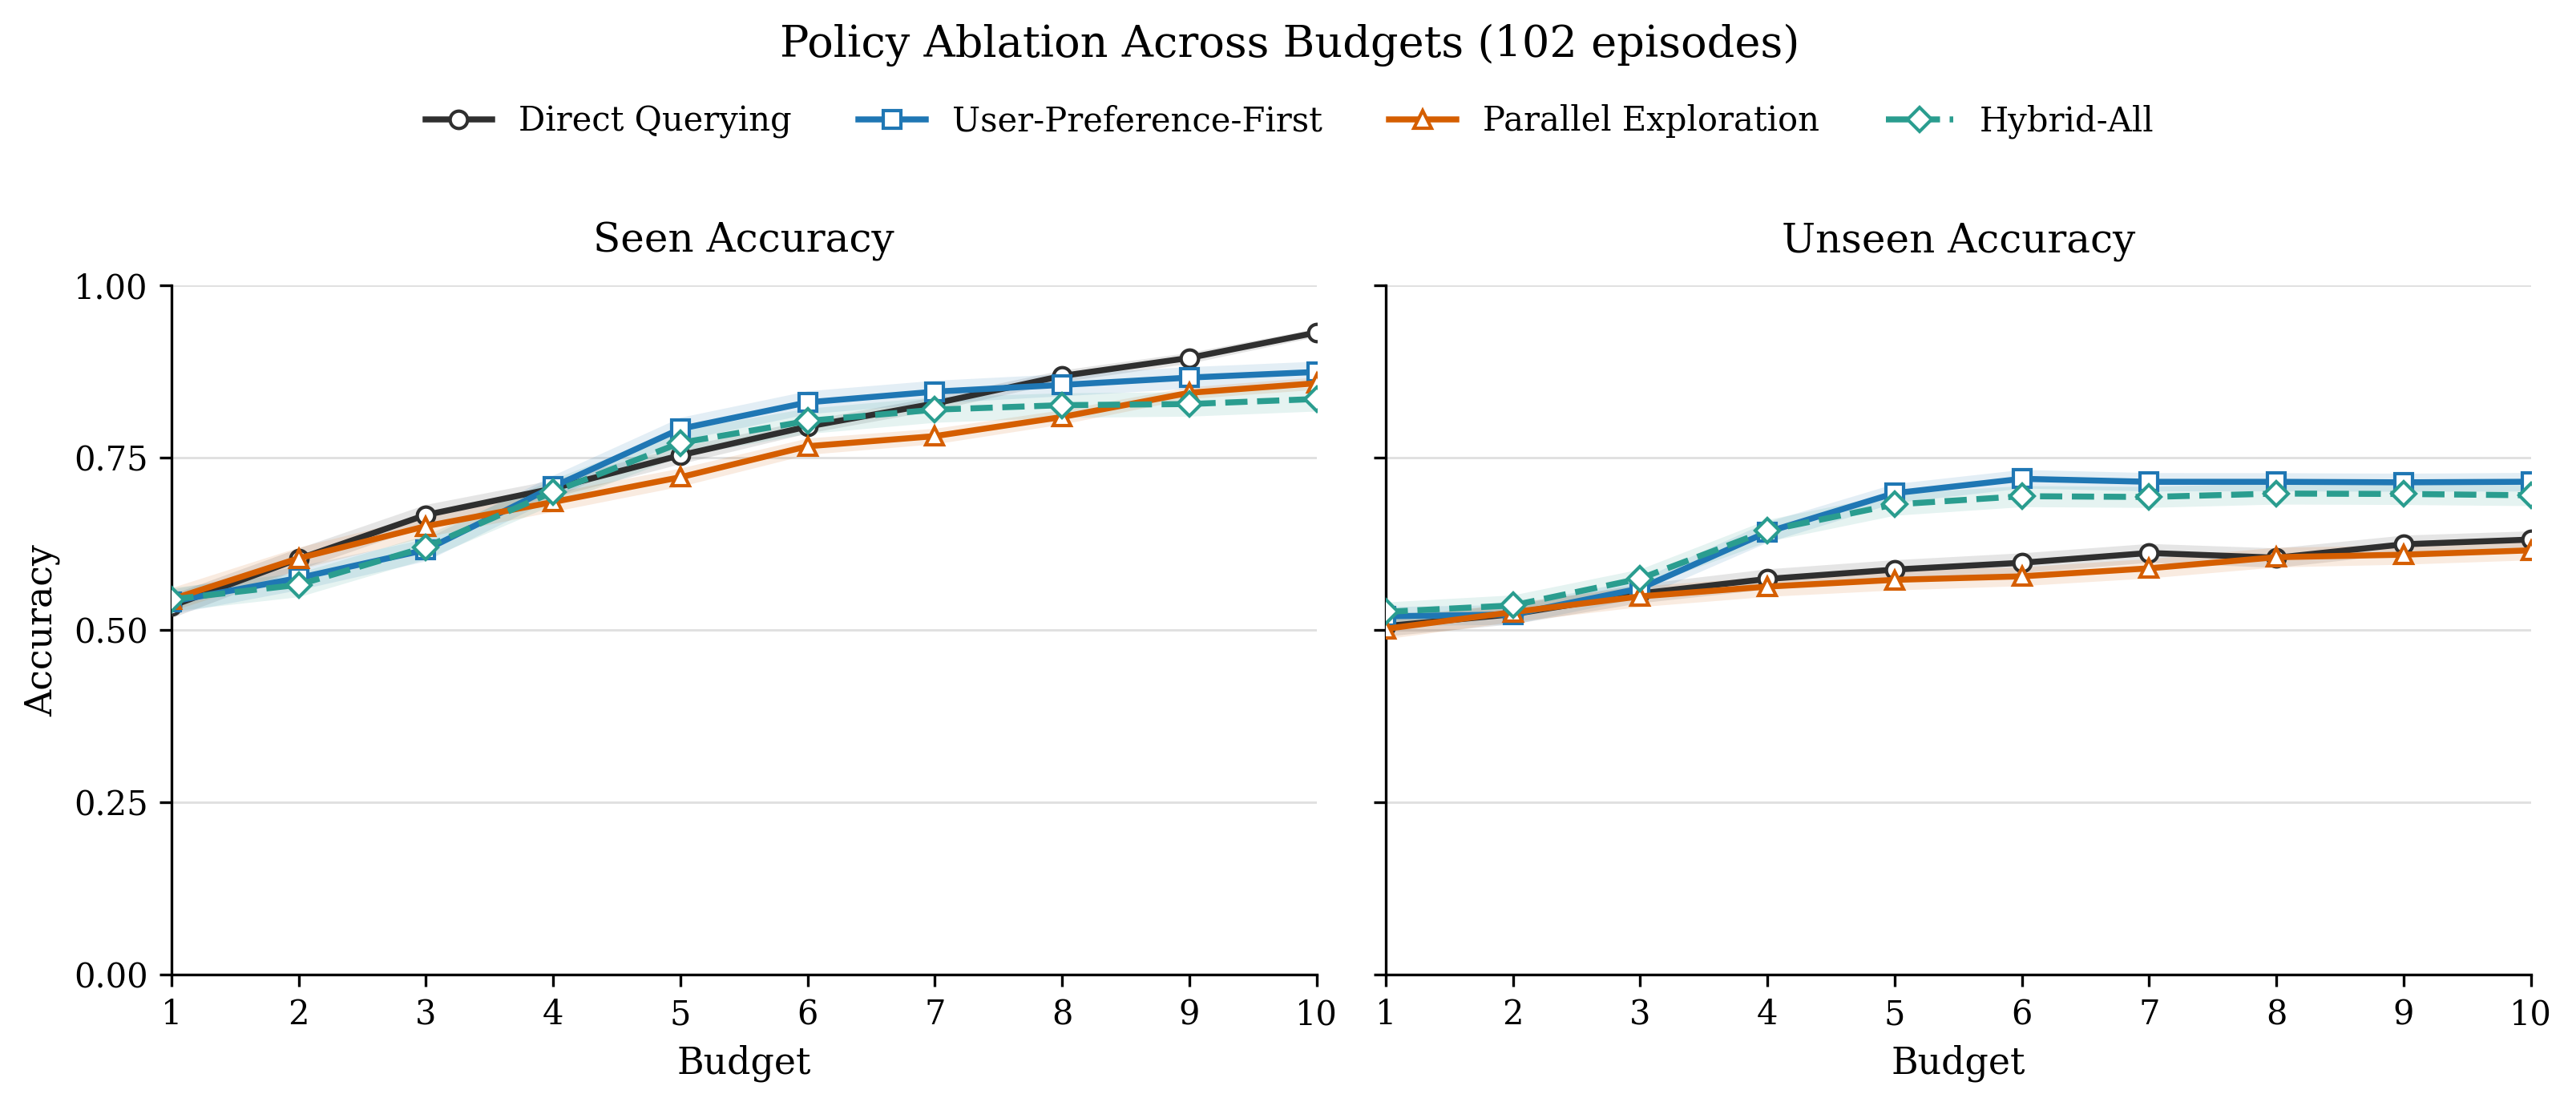
\includegraphics[width=\textwidth]{../plots/ablation_full_qwen3.png}
\caption{Seen and unseen accuracy by policy mode across question budgets $B=1$--$10$ (102 episodes, Qwen3). Shaded regions indicate $\pm$1 standard error. UPF and HYB separate sharply from DQ and PAR on unseen accuracy beginning at $B=4$.}\label{fig:main_results}
\end{figure}

\subsubsection{Hypothesis Evaluation}

\paragraph{H1 supported: Preference-based policies substantially outperform direct querying on unseen objects.}
UPF achieves 69.8\% unseen accuracy at $B=5$, compared to DQ's 58.7\%---a gap of 11.1 percentage points ($p < .001$, paired $t$-test). HYB shows a similar advantage (+9.5pp). The gap persists across all budgets $B \geq 4$ and is consistent across room types. Category-level rules learned through PE generalize to unseen objects in ways that object-level confirmed actions cannot (H1 confirmed).

\paragraph{H2 supported: The UPF--DQ gap widens with budget, then plateaus.}
At $B=1$--$3$, all four policies perform comparably on unseen accuracy (50--56\%). The gap opens at $B=4$ when UPF begins covering multiple receptacles with PE rules: by $B=5$, UPF leads DQ by 11.1pp. The gap stabilizes at $B=6$--$10$ as UPF saturates coverage of all 5 receptacles. Each PE question covers one receptacle; with 5 receptacles, $B=5$ is sufficient for full coverage. Additional budget provides diminishing returns through AO boundary probing (H2 confirmed).

\paragraph{H3 supported: DQ provides faster seen-object gains at low budgets.}
At $B=1$, DQ seen accuracy (53.4\%) matches UPF (54.1\%). By $B=10$, DQ reaches 93.1\% seen accuracy---the highest among all policies---because every question directly resolves one object. UPF seen accuracy plateaus at 87.4\%, since PE questions resolve objects only indirectly through category inference. For seen objects specifically, direct querying remains the most efficient approach (H3 confirmed).

\paragraph{H4 supported: Bottom-up induction is less efficient than top-down elicitation.}
PAR's do-and-induce cycle (AO$\to$AO$\to$PI) produces approximately 2--3 confirmed preferences per 10 budget steps, compared to UPF's 5 (one PE per receptacle). PAR's unseen accuracy (61.5\% at $B=10$) is statistically indistinguishable from DQ (63.1\%), confirming that the overhead of accumulating evidence before inducing a rule negates the generalization benefit of the induced rule itself. The structural disadvantage is clear: PAR requires $\sim$3 questions per rule versus UPF's 1 (H4 confirmed).

\paragraph{H5 supported: Hybrid performs comparably to UPF.}
HYB's unseen accuracy closely tracks UPF across all budgets (within 2pp), confirming that the additional flexibility of combining PE, AO, and PI does not provide a meaningful advantage over UPF's simpler PE-first policy. Both policies achieve similar coverage because their primary mechanism---PE for receptacle rule discovery---is identical. The main difference is that HYB occasionally uses PI for consolidation, which provides marginal benefit (H5 confirmed).

\subsubsection{Cross-Model Validation}

To assess whether findings generalize beyond a single LLM, we replicated the experiment on a 10-episode subset using GPT-5-chat (OpenAI API). The UPF advantage over DQ was even larger (+15.0pp at $B=5$), consistent with the hypothesis that stronger LLMs amplify the benefit of category-level rules by improving both PE question quality and finalizer reasoning. The policy ranking (UPF $\approx$ HYB $>$ DQ $\approx$ PAR) was preserved across both models.

\subsubsection{Implications for Study~2}

The simulation establishes that UPF and DQ represent meaningfully distinct strategies: UPF excels at generalization through category-level rules, while DQ excels at seen-object resolution through direct evidence. PAR's near-parity with DQ despite using PI suggests that the value of preference rules depends critically on \emph{how} they are acquired---direct elicitation (PE) is far more effective than bottom-up induction (PI) in this setting. Whether these performance differences translate into user experience differences---and whether real users can articulate category-level rules as reliably as the oracle---requires human participants. Study~2 addresses these questions.

\subsection{Limitations of Simulated Evaluation}

The oracle provides consistent, well-formed answers using exact receptacle names---a best-case scenario. Real users may give ambiguous, incomplete, or multi-part answers, especially in response to PE's abstract questions. The simulation does not model frustration, hedging, or changing mental representations during the interaction. Additionally, the LLM-based state update module occasionally misclassifies objects when category boundaries overlap (e.g., a ``plastic toy bin'' categorized as a ``play item'' rather than ``storage container''), which affects all policies equally. Study~2 directly addresses these limitations.


% ============================================================
% 5. STUDY 2: HOW QUESTIONING STRATEGIES AFFECT USER EXPERIENCE
% ============================================================
\section{Study 2: How Questioning Strategies Affect User Experience}\label{sec:study2}

\TODO{This section presents the user study design and results. The subsections below provide the planned structure; content will be completed after data collection.}

\subsection{Research Questions and Hypotheses}

Study~2 investigates the experiential dimensions of questioning strategy that are not accessible through simulation. Guided by the theoretical framing in Section~\ref{sec:related} and the simulation findings of Study~1, we examine:

\begin{enumerate}[label=\textbf{RQ\arabic*:},leftmargin=*]
    \item[RQ3.] How do strategies differ in perceived control, cognitive load, trust, and satisfaction?
    \item[RQ4.] Does organizing expertise moderate strategy effectiveness?
\end{enumerate}

We formulate additional hypotheses:

\begin{description}[leftmargin=*]
    \item[\textbf{H6}] PE questioning will produce lower perceived control than AO, because abstract category questions reduce users' sense of moment-to-moment agency over placement decisions.
    \item[\textbf{H7}] AO questioning will produce higher cognitive load ratings at higher budgets than PE, because resolving objects one-by-one becomes tedious relative to category-level resolution.
    \item[\textbf{H8}] Users with high organizing expertise will prefer PE (able to articulate abstract rules), while users with low expertise will prefer AO (concrete, low cognitive demand).
\end{description}

\subsection{Study Design}

\TODO{Within-subject design. Each participant experiences 2--3 strategy conditions (counterbalanced using a Latin square). Independent variable: questioning strategy (AO / PE / Combined). Question budget fixed at $B=6$ to match Study~1's highest-budget condition.}

\subsection{Participants}

\TODO{Target: 24--30 participants. Recruitment via university participant pool and community posting. Inclusion criteria: age 18--65, resident of a private home for at least 6 months. Organizing expertise assessed via 5-item self-report scale (``I have specific rules for where household items belong'', 1--5 Likert). IRB approval obtained from [institution].}

\subsection{Task and Procedure}

\TODO{Participants interact with the agent through a web-based chat interface to organize a virtual room (12 seen + 12 unseen objects, same room types as Study~1). Each session: self-introduction + organizing expertise questionnaire $\to$ condition 1 interaction (budget=6) $\to$ post-condition questionnaire $\to$ repeat for conditions 2 and 3 $\to$ comparative preference interview. Three distinct room types used across conditions to minimize learning effects. Condition order counterbalanced.}

\subsection{Interface}

\TODO{Web chat interface. Agent presents questions; user types free-text responses. Room state displayed as a labelled diagram showing current placements in real time. All interactions, timestamps, and intermediate agent state logged. Pilot test with 3 users to verify interface usability.}

\subsection{Measures}

\subsubsection{Task Performance}
Seen accuracy and unseen accuracy (same definition as Study~1), enabling direct comparison with simulation results. Objects per question (information efficiency).

\subsubsection{User Experience Questionnaire}
\TODO{Post-condition questionnaire: NASA-TLX (cognitive load, 6 subscales); perceived control (5 items adapted from \citealt{skjuve2025chatgpt}); trust in agent (5 items adapted from \citealt{mahmood2025user}); satisfaction (1 item, 7-point scale). Comparative preference interview: ``Which style did you prefer and why?'', ``Did you feel in control?'', ``Were any questions confusing?''}

\subsubsection{Interaction Logs}
\TODO{Response length per answer, answer hesitation (time from question display to first keystroke), number of follow-up clarifications requested.}

\subsection{Analysis Plan}

\TODO{Quantitative: linear mixed-effects models with strategy as within-subject factor and organizing expertise as continuous covariate, allowing strategy $\times$ expertise interaction to test H8. Random intercept per participant. Qualitative: thematic analysis of interview transcripts using reflexive coding \citep{braun2019thematic}; two coders, Cohen's $\kappa$ reported.}

\subsection{Results}

\subsubsection{Task Performance with Real Users}
\TODO{Compare seen and unseen accuracy per strategy. Expected: PE $>$ AO for unseen accuracy, consistent with H3. Real users may give less precise answers, narrowing the gap. Raw LLM condition repeated if feasible.}

\subsubsection{User Experience Across Strategies}
\TODO{Report mixed-effects results for each outcome measure. Expected: PE lower perceived control (H6), AO higher cognitive load at $B=6$ (H7). Present effect sizes; discuss practical significance alongside statistical significance.}

\subsubsection{The Role of Organizing Expertise}
\TODO{Report strategy $\times$ expertise interaction effects. Expected: experts prefer PE; novices prefer AO (H8). Illustrate with representative quotes from interviews.}

\subsubsection{Interaction Patterns and Breakdowns}
\TODO{Qualitative themes: when do users give multi-receptacle answers to PE questions? When do users reject PI hypotheses and why? What conversational repair strategies emerge? How do users express uncertainty? These patterns extend the simulation findings by exposing real user behaviors that the oracle cannot replicate.}


% ============================================================
% 6. DISCUSSION
% ============================================================
\section{Discussion}\label{sec:discussion}

\subsection{Simulation Versus Real User Behavior: Where the Gap Lies}

\TODO{Study~1 establishes that PE's category-level rules dramatically improve generalization in an ideal oracle environment. Study~2 will reveal whether this advantage persists when users give ambiguous answers, answer at varying levels of specificity, or misinterpret abstract questions. We anticipate that the PE--AO accuracy gap will narrow with real users---the interesting question is \emph{by how much} and \emph{which user characteristics} determine the size of the gap. If expert organizers preserve PE's accuracy advantage while novices do not, this directly supports an adaptive strategy recommendation.}

\subsection{The Accuracy--Agency Trade-off}

\TODO{Discuss the tension between information efficiency (PE) and user agency (AO). Category-level questions are more efficient but implicitly ask the user to accept the agent's framing of their organizing categories---which may not match their actual mental model. Concrete object questions are less efficient but position the user as the definitive authority. This trade-off mirrors findings in conversational recommendation \citep{shin2025toward} where personalizing the interaction modality to user preferences improved both outcomes and satisfaction.}

The trade-off also has a temporal dimension: at low budgets ($B \leq 2$), AO and PE are nearly equivalent on seen accuracy. The accuracy cost of choosing AO over PE is small when only a few questions are permitted. Designers who prioritize user agency can reasonably default to AO for short interactions---using PE only when a larger question budget is available and the generalization benefit justifies asking users to reason more abstractly about their preferences.

\subsection{Theoretical Contributions}

\TODO{This work contributes three main theoretical claims:
(1) The granularity of preference queries---not just their presence---determines the type and generalizability of learned preferences; the AO/PE/PI taxonomy captures this granularity across a dimension not previously formalized in the literature.
(2) Structured state representation (confirmed actions and preferences as typed records) provides consistent accuracy benefits over raw dialogue history retention, suggesting that intermediate representation---not just language model scaling---is important for preference-learning agents.
(3) Organizing expertise is a theoretically principled moderator of questioning strategy effectiveness: it predicts users' ability to respond usefully to abstract category questions. This extends the finding of \citet{skjuve2025chatgpt} that user experience level moderates LLM interaction quality into the domain of preference elicitation.}

\subsection{Design Recommendations}

Based on the simulation evidence from Study~1 and the predicted findings of Study~2, we offer four recommendations for designers of conversational agents that learn user preferences:

\begin{enumerate}[leftmargin=*]
    \item \textbf{Open with category-level questions when budget allows.} PE's compounding accuracy advantage is maximized over more questions. An agent with a budget of 4 or more should begin with PE to establish broad rules, then fall back to AO for remaining ambiguities.
    \item \textbf{Match questioning granularity to user expertise.} Users who struggle to articulate organizing principles in category-level terms should be offered the more concrete AO style; users who readily express general rules stand to benefit more from PE's higher information yield. A brief initial exchange---or a simple self-report item---can inform this routing.
    \item \textbf{Maintain structured preference records rather than raw dialogue.} Confirmed actions and preferences with explicit receptacle associations substantially outperform free-form dialogue retention for downstream placement. The gains are especially large for unseen objects, where the agent cannot rely on direct recall of a prior answer.
    \item \textbf{Give users explicit control over questioning style.} Because strategies differ in how much agency users feel over placement decisions, offering a brief framing at the start of the interaction (``I can ask you about specific items, or about your general organizing habits---which would you prefer?'') respects user autonomy and may improve satisfaction without sacrificing accuracy.
\end{enumerate}

\subsection{Limitations}

Four limitations bound the scope of the current findings. First, the simulated oracle represents a best-case user: consistent, precise, and fluent with exact receptacle names. Real users give more varied responses, and Study~2 will begin to characterize that variability---but even a lab user study captures a narrow demographic and cultural context. The norms governing ``where things belong'' vary substantially across households and cultures; whether our strategy taxonomy generalizes across those norms is an open question.

Second, the evaluation covers three room types (living room, bedroom, kitchen) representing prototypical residential spaces. Strategies may behave differently in more specialized environments (home offices, workshops, shared spaces) or in rooms with ambiguous or overlapping receptacle categories.

Third, all reported results use a single LLM backend (Qwen3). The proposer and state-update modules depend on the model's ability to generate well-formed structured outputs; performance may vary with model capability, temperature settings, or prompt design. Replication with alternative models is needed before generalizing the quantitative findings.

Fourth, both the simulation and the planned user study are single-session. Household preferences are not static: users learn, reorganize, and develop new habits over time. A longitudinal evaluation---where the agent refines its preference model across multiple sessions---would provide a more ecologically valid test of each strategy's long-term utility.

\subsection{Future Directions}

Several extensions follow naturally from this work. Adaptive policy selection---dynamically choosing among AO, PE, and PI based on accumulated uncertainty estimates (e.g., entropy reduction per expected question)---is a principled next step that our structured state representation already supports. Deployment on a physical robot would introduce perception noise and real-world object variability, testing the limits of preference generalization in a way that simulation cannot. Longitudinal multi-session studies would examine how learned preferences persist and evolve. Finally, pre-registered, larger-scale user studies would provide higher-powered tests of the expertise moderation hypothesis (H8) and the design recommendations derived from it.


% ============================================================
% 7. CONCLUSION
% ============================================================
\section{Conclusion}\label{sec:conclusion}

We investigated how an intelligent agent should ask for user preferences when assisting with household rearrangement. Grounding the investigation in three questioning patterns---Action-Oriented, Preference Eliciting, and Preference Induction---composed into four dialogue policies, we showed that the \emph{how} of asking has consequences that extend far beyond information efficiency.

Simulation across 102 household episodes with budgets 1--10 established three key findings. First, the User-Preference-First policy (PE then AO boundary probing) achieves 69.8\% unseen accuracy at $B=5$, outperforming Direct Querying by 11.1 percentage points, because category-level rules transfer directly to novel objects. Second, the Parallel Exploration policy (AO then PI induction) fails to outperform Direct Querying despite using the same budget, revealing that the \emph{acquisition method}---not merely the presence of rules---determines generalization benefit: top-down elicitation is far more efficient than bottom-up induction (1 question per rule vs.\ $\sim$3). Third, the advantage of preference-first questioning emerges at $B \geq 4$ and plateaus at $B \geq 6$, providing clear guidance for budget allocation in practice. Cross-model validation with GPT-5 preserves the policy ranking while amplifying the preference-first advantage.

\TODO{Study~2 will further reveal how these performance differences translate to user experience: which policy users prefer, when they feel in control, and how organizing expertise shapes those judgments.}

Together, these findings establish that dialogue policy design---the sequencing and composition of questioning patterns---fundamentally shapes the quality of learned preferences and their generalizability. The question of how to ask, not just what to ask, is a first-class design decision for conversational agents that learn from users.


% ============================================================
% REFERENCES
% ============================================================
\bibliographystyle{cas-model2-names}
\bibliography{cas-refs}

% ============================================================
% APPENDIX
% ============================================================
\appendix

\section{Prompt Templates}\label{app:prompts}
\TODO{Include key prompt templates for each strategy's proposer, state update interpreter, and final placement planner. Representative examples of oracle answers for each strategy type. This supports reproducibility.}

\section{Dataset Statistics}\label{app:dataset}
\TODO{Table: distribution of objects per receptacle across room types. Table: receptacle set size by room. Examples of annotator notes per room type. Inter-annotator agreement if applicable.}

\section{User Study Materials}\label{app:userstudy}
\TODO{Pre-task questionnaire (demographics, organizing expertise scale). Post-condition questionnaire (NASA-TLX, perceived control, trust, satisfaction). Semi-structured interview protocol. Informed consent form. Counterbalancing schedule.}

\end{document}
